\subsection{Bài tập về thiết bị khuấy trộn liên tục}
\subsubsection{Mô hình về thiết bị khuấy trộn liên tục}
    \begin{figure}[htp]
        \begin{center}
            \subfloat[Mô hình 1 \label{Fig:binhchuachatlong-khuaytron-mohinh1}]
                {
                    \subimport{section/mohinhhoalythuyet/images/}{binhchuachatlong-khuaytron-mohinh1.tex}
                }
            \subfloat[Mô hình 2 \label{Fig:binhchuachatlong-khuaytron-mohinh2}]
                {
                    \subimport{section/mohinhhoalythuyet/images/}{binhchuachatlong-khuaytron-mohinh2.tex}
                }
            % \subfloat[Mô hình 3 \label{Fig:binhchuachatlong-khuaytron-mohinh3}]
            %     {
            %         \subimport{section/mohinhhoalythuyet/images/}{binhchuachatlong-khuaytron-mohinh3.tex}
            %     }
        \end{center}
        \caption{Các mô hình về thiết bị khuấy trộn liên tục} \label{Fig:binhchuachatlong-khuaytron}
    \end{figure}

\subparagraph{Các đại lượng trên mô hình}
    \begin{itemize}
		\item $w_1, w_2$: Lưu lượng khối lượng nguyên liệu của hai dòng nguyên liệu $\pfm{kg/s}$ hoặc $\pfm{kg/\text{\textit{phút}}}$.
		\item $x_1, x_2$: Thành phần của 2 dòng nguyên liệu.
		\item $w$: Lưu lượng khối lượng dòng sản phẩm ra $\pfm{kg/s}$ hoặc $\pfm{kg/\text{\textit{phút}}}$.
		\item $x$: Thành phần của sản phẩm ra.
		\item $h$: Mức chất lỏng trong bình $\pfm{m}$.
	\end{itemize}

\subparagraph{Mô tả quá trình} Hai dòng nguyên liệu có thành phần chất $A$ lần lượt là $x_1$ và $x_2$ được đưa vào thiết bị khuấy trộn, tạo ra một dòng sản phẩm có nồng độ $x$ theo yêu cầu. Lưu lượng dòng nguyên liệu được điều khiển qua các van. Quá trình pha chế được hỗ trợ bởi một hệ thống khuấy trộn gắn động cơ.

\subsubsection{Xác định các biến quá trình}
    \begin{itemize}
        \item Mô hình trong \fig{\ref{Fig:binhchuachatlong-khuaytron-mohinh1}}:
            \begin{center}
                \begin{tabular}{l|l}
                    Biến vào: $x_1, x_2$ và $w, w_1, w_2$ & Biến điều khiển: $w_1,w_2$ \\ \hline
                    Biến ra: $x,h$ & Biến cần điều khiển: $x,h$\\ \hline
                    & Biến nhiễu: $x_1, x_2$ và $w$
                \end{tabular}
            \end{center}

        \item Mô hình trong \fig{\ref{Fig:binhchuachatlong-khuaytron-mohinh2}}:
            \begin{center}
                \begin{tabular}{l|l}
                    Biến vào: $x_1, x_2$ và $w, w_1, w_2$ & Biến điều khiển: $w, w_1$ \\ \hline
                    Biến ra: $x,h$ & Biến cần điều khiển: $x,h$\\ \hline
                    & Biến nhiễu: $x_1, x_2$ và $w_2$
                \end{tabular}
            \end{center}
    \end{itemize}

\subsubsection{Xây dựng phương trình toán học}
    \begin{itemize}
        \item Giả thiết:
            \begin{itemize}
                \item Bỏ qua trễ do vận chuyển.
                \item Quá trình khuấy trộn được xem là lý tưởng, chất lỏng đồng nhất tại mọi vị trí trong thiết bị.
                \item Khối lượng riêng của hỗn hợp trong thiết bị được coi là thay đổi không đáng kể.
            \end{itemize}
        \item Công thức tính thể tích $V = Ah$ với $A$ là tiết diện của bình chứa.
        \item Áp dụng phương trình cân bằng vật chất:
            \begin{align*}
                \rho \dfrac{dV}{dt} = w_1 + w_2 - w \Longleftrightarrow \rho \dfrac{d\pfm{Ah}}{dt} = w_1 + w_2 - w \Longleftrightarrow \dfrac{dh}{dt} = \dfrac{1}{\rho A} \pfm{w_1 + w_2 - w}
            \end{align*}
        \item Phương trình cân bằng thành phần:
            \begin{align*}
                \rho \dfrac{d\pfm{Vx}}{dt} = w_1x_1 + w_2x_2 - wx
            \end{align*}
        \item Khai triển đạo hàm riêng cho vế trái, ta có phương trình:
            \begin{align*}
                & \rho V \dfrac{dx}{dt} + \rho x \dfrac{dV}{dt} = w_1x_1 + w_2x_2 - wx\\
                \Longleftrightarrow~ & \rho V \dfrac{dx}{dt} + x \pfm{w_1 + w_2 - w} = w_1x_1 + w_2x_2 - wx\\
                \Longleftrightarrow~ & \rho V \dfrac{dx}{dt} = w_1x_1 + w_2x_2 - \pfm{w_1 + w_2}x\\
                \Longleftrightarrow~ & \dfrac{dx}{dt} = \dfrac{1}{\rho V} \left[{w_1x_1 + w_2x_2 - \pfm{w_1 + w_2}x}\right]\\
                \Longleftrightarrow~ & \dfrac{dx}{dt} = \dfrac{1}{\rho A h} \left[{w_1x_1 + w_2x_2 - \pfm{w_1 + w_2}x}\right]
            \end{align*}
        \item Kết luận, mô hình toán của hệ thống là:
            \begin{align*}
                \left\{\begin{array}{l}
                    \dfrac{dh}{dt}  = \dfrac{1}{\rho A} \pfm{w_1 + w_2 - w}\\
                    \dfrac{dx}{dt}  = \dfrac{1}{\rho A h} \left[{w_1x_1 + w_2x_2 - \pfm{w_1 + w_2}x}\right]
                \end{array}\right.
            \end{align*}
    \end{itemize}

\subsubsection{Tuyến tính hóa phương trình quanh điểm làm việc cân bằng}
    \begin{itemize}
        \item Đặt: $h = \overline{h} + \Delta h$; $x = \overline{x} + \Delta x$; $w_1 = \overline{w}_1 + \Delta w_1$; $w_2 = \overline{w}_2 + \Delta w_2$; $w = \overline{w} + \Delta w$; $x_1 = \overline{x}_1 + \Delta x_1$; $x_2 = \overline{x}_2 + \Delta x_2$.
        \item Tại điểm làm việc cân bằng $(\overline{h}, \overline{x}, \overline{x}_1, \overline{x}_2, \overline{w}_1, \overline{w}_2, \overline{w})$, ta có:
            \begin{align*}
                \left\{\begin{array}{l}
                    \dfrac{dh}{dt}  = \dfrac{1}{\rho A} \pfm{\overline{w}_1 + \overline{w}_2 - \overline{w}} = 0 \\
                    \dfrac{dx}{dt}  = \dfrac{1}{\rho A \overline{h}} \left[{\overline{w}_1 \overline{x}_1 + \overline{w}_2 \overline{x}_2 - \pfm{\overline{w}_1 + \overline{w}_2}\overline{x}}\right] = 0
                \end{array}\right.
                \Longleftrightarrow
                \left\{\begin{array}{l}
                     \overline{w}_1 + \overline{w}_2 = \overline{w} \\
                    \overline{w}_1\overline{x}_2 + \overline{w}_2\overline{x}_2 - \pfm{\overline{w}_1 + \overline{w}_2}\overline{x} = 0
                \end{array}\right.
            \end{align*}
        \item Ta có: $\dfrac{dh}{dt}  = \dfrac{1}{\rho A} \pfm{w_1 + w_2 - w}$ đã tuyến tính hóa, nên:
            \begin{align*}
                \dot{h} = \Delta \dot{h} = \dfrac{1}{\rho A} \pfm{\Delta w_1 + \Delta w_2 - \Delta w}
            \end{align*}
        \item Khai triển Taylor cho $f(h, x, x_1, x_2, w_1, w_2, w) = \dfrac{dx}{dt}  = \dfrac{1}{\rho A h} \left[{w_1x_1 + w_2x_2 - \pfm{w_1 + w_2}x}\right]$ tại điểm làm việc cân bằng $(\overline{h}, \overline{x}, \overline{x}_1, \overline{x}_2, \overline{w}_1, \overline{w}_2, \overline{w})$, ta có:
            \begin{align*}
                \dot{x} = \Delta \dot{x} = & \underbrace{f(\overline{h}, \overline{x}, \overline{x}_1, \overline{x}_2, \overline{w}_1, \overline{w}_2, \overline{w})}_{0} + \dfrac{df}{dh}\Delta h + \dfrac{df}{dx}\Delta x + \dfrac{df}{dx_1}\Delta x_1 + \dfrac{df}{dx_2}\Delta x_2 + \dfrac{df}{dw_1}\Delta w_1 \\
                & + \dfrac{df}{dw_2}\Delta w_2 + \dfrac{df}{dw}\Delta w \\
                = & \dfrac{-1}{\rho A \overline{h}^2} \underbrace{\left[{\overline{w}_1 \overline{x}_1 + \overline{w}_2 \overline{x}_2 - \pfm{\overline{w}_1 + \overline{w}_2}\overline{x}}\right]}_{0} \Delta h + \dfrac{-1}{\rho A \overline{h}} \underbrace{\pfm{\overline{w}_1 + \overline{w}_2}}_{\overline{w}} \Delta x + \dfrac{\overline{w}_1}{\rho A \overline{h}} \Delta x_1 + \dfrac{\overline{w}_2}{\rho A \overline{h}} \Delta x_2 \\
                & + \dfrac{\overline{x}_1 - \overline{x}}{\rho A \overline{h}} \Delta w_1 + \dfrac{\overline{x}_2 - \overline{x}}{\rho A \overline{h}} \Delta w_2 + 0\\
                = & - \dfrac{\overline{w}}{\rho A \overline{h}} \Delta x + \dfrac{\overline{w}_1}{\rho A \overline{h}} \Delta x_1 + \dfrac{\overline{w}_2}{\rho A \overline{h}} \Delta x_2 + \dfrac{\overline{x}_1 - \overline{x}}{\rho A \overline{h}} \Delta w_1 + \dfrac{\overline{x}_2 - \overline{x}}{\rho A \overline{h}} \Delta w_2
            \end{align*}
        \item Kết luận, mô hình tuyến tính hóa theo khai triển Taylor có dạng:
            \begin{align*}
                \left\{\begin{array}{l}
                    \Delta \dot{h} = \dfrac{1}{\rho A} \pfm{\Delta w_1 + \Delta w_2 - \Delta w}\\
                    \Delta \dot{x} = - \dfrac{\overline{w}}{\rho A \overline{h}} \Delta x + \dfrac{\overline{w}_1}{\rho A \overline{h}} \Delta x_1 + \dfrac{\overline{w}_2}{\rho A \overline{h}} \Delta x_2 + \dfrac{\overline{x}_1 - \overline{x}}{\rho A \overline{h}} \Delta w_1 + \dfrac{\overline{x}_2 - \overline{x}}{\rho A \overline{h}} \Delta w_2
                \end{array}\right.
            \end{align*}
    \end{itemize}

\subsubsection{Xây dựng hàm truyền và vẽ sơ đồ khối mô tả quá trình}
    \begin{itemize}
        \item Ta có $\Delta \dot{h} = \dfrac{1}{\rho A} \pfm{\Delta w_1 + \Delta w_2 - \Delta w}$, khai triển Laplace:
            \begin{align*}
                & s \Delta H(s) = \dfrac{1}{\rho A} \left[{\Delta W_1(s) + \Delta W_2(s) - \Delta W(s)}\right]\\
                \Longleftrightarrow & \Delta H(s) = \dfrac{1}{\rho As} \Delta W_1(s) + \dfrac{1}{\rho As} \Delta W_2(s) - \dfrac{1}{\rho As} \Delta W(s)
            \end{align*}

        \item Đặt $k_{wh} = \dfrac{1}{\rho A}$, ta có: $\Delta H(s) = \dfrac{k_{wh}}{s} \Delta W_1(s) + \dfrac{k_{wh}}{s} \Delta W_2(s) - \dfrac{k_{wh}}{s} \Delta W(s)$
        \item Ta có $\Delta \dot{x} = - \dfrac{\overline{w}}{\rho A \overline{h}} \Delta x + \dfrac{\overline{w}_1}{\rho A \overline{h}} \Delta x_1 + \dfrac{\overline{w}_2}{\rho A \overline{h}} \Delta x_2 + \dfrac{\overline{x}_1 - \overline{x}}{\rho A \overline{h}} \Delta w_1 + \dfrac{\overline{x}_2 - \overline{x}}{\rho A \overline{h}} \Delta w_2$, khai triển Laplace:
            \begin{align*}
                & s X(s) = - \dfrac{\overline{w}}{\rho A \overline{h}} \Delta X(s) + \dfrac{\overline{w}_1}{\rho A \overline{h}} \Delta X_1(s) + \dfrac{\overline{w}_2}{\rho A \overline{h}} \Delta X_2(s) + \dfrac{\overline{x}_1 - \overline{x}}{\rho A \overline{h}} \Delta W_1(s) + \dfrac{\overline{x}_2 - \overline{x}}{\rho A \overline{h}} \Delta W_2(s) \\
                \Longleftrightarrow & \rho A \overline{h} s X(s) + \overline{w} \Delta X(s) = \overline{w}_1 \Delta X_1(s) + \overline{w}_2 \Delta X_2(s) + \pfm{\overline{x}_1 - \overline{x}} \Delta W_1(s) + \pfm{\overline{x}_2 - \overline{x}} \Delta W_2(s)\\
                \Longleftrightarrow & \pfm{\dfrac{\rho A \overline{h}}{\overline{w}}s + 1}\Delta X(s) = \dfrac{\overline{w}_1}{\overline{w}} \Delta X_1(s) + \dfrac{\overline{w}_2}{\overline{w}} \Delta X_2(s) + \dfrac{\overline{x}_1 - \overline{x}}{\overline{w}} \Delta W_1(s) + \dfrac{\overline{x}_2 - \overline{x}}{\overline{w}} \Delta W_2(s)
            \end{align*}
        \item Đặt $\tau = \dfrac{\rho A \overline{h}}{\overline{w}}$; $k_{x1x} = \dfrac{\overline{w}_1}{\overline{w}}$; $k_{x2x} = \dfrac{\overline{w}_2}{\overline{w}}$; $k_{w1x} = \dfrac{\overline{x}_1 - \overline{x}}{\overline{w}}$; $k_{w2x} = \dfrac{\overline{x}_2 - \overline{x}}{\overline{w}}$, ta có:
            \begin{align*}
                & \pfm{\tau s + 1}\Delta X(s) = k_{x1x} \Delta X_1(s) + k_{x2x} \Delta X_2(s) + k_{w1x} \Delta W_1(s) + k_{w2x} \Delta W_2(s) \\
                \Longleftrightarrow & \Delta X(s) = \dfrac{k_{x1x}}{\tau s + 1} \Delta X_1(s) + \dfrac{k_{x2x}}{\tau s + 1} \Delta X_2(s) + \dfrac{k_{w1x}}{\tau s + 1} \Delta W_1(s) + \dfrac{k_{w2x}}{\tau s + 1} \Delta W_2(s)
            \end{align*}
        \item Kết luận:
            \begin{align*}
                \left\{\begin{array}{l}
                    \Delta H(s) = \dfrac{k_{wh}}{s} \Delta W_1(s) + \dfrac{k_{wh}}{s} \Delta W_2(s) - \dfrac{k_{wh}}{s} \Delta W(s)\\
                    \Delta X(s) = \dfrac{k_{x1x}}{\tau s + 1} \Delta X_1(s) + \dfrac{k_{x2x}}{\tau s + 1} \Delta X_2(s) + \dfrac{k_{w1x}}{\tau s + 1} \Delta W_1(s) + \dfrac{k_{w2x}}{\tau s + 1} \Delta W_2(s)\\
                    k_{wh} = \dfrac{1}{\rho A}; \tau = \dfrac{\rho A \overline{h}}{\overline{w}}; k_{x1x} = \dfrac{\overline{w}_1}{\overline{w}}; k_{x2x} = \dfrac{\overline{w}_2}{\overline{w}}; k_{w1x} = \dfrac{\overline{x}_1 - \overline{x}}{\overline{w}}; k_{w2x} = \dfrac{\overline{x}_2 - \overline{x}}{\overline{w}}
                \end{array}\right.
            \end{align*}

        \item Ta có các hàm truyền mô tả hệ thống như sau:
            \begin{align*}
                \left\{\begin{array}{l}
                    \dfrac{H(s)}{W_1(s)} = \dfrac{k_{wh}}{s}; \dfrac{H(s)}{W_2(s)} = \dfrac{k_{wh}}{s}; \dfrac{H(s)}{W(s)} = -\dfrac{k_{wh}}{s}; \dfrac{H(s)}{X_1(s)} = 0; \dfrac{H(s)}{X_2(s)} = 0\\
                    \dfrac{X(s)}{W_1(s)} = \dfrac{k_{w1x}}{\tau s + 1}; \dfrac{X(s)}{W_2(s)} = \dfrac{k_{w2x}}{\tau s + 1}; \dfrac{X(s)}{X_1(s)} = \dfrac{k_{x1x}}{\tau s + 1}; \dfrac{X(s)}{X_2(s)} = \dfrac{k_{x2x}}{\tau s + 1}; \dfrac{X(s)}{W(s)} = 0 \\
                    k_{wh} = \dfrac{1}{\rho A}; \tau = \dfrac{\rho A \overline{h}}{\overline{w}}; k_{x1x} = \dfrac{\overline{w}_1}{\overline{w}}; k_{x2x} = \dfrac{\overline{w}_2}{\overline{w}}; k_{w1x} = \dfrac{\overline{x}_1 - \overline{x}}{\overline{w}}; k_{w2x} = \dfrac{\overline{x}_2 - \overline{x}}{\overline{w}}
                \end{array}\right.
            \end{align*}

    \item Giả thiết: thiết bị khuấy trộn liên tục có tiết diện đều $A = 0.8\unit{m^2}$ và khối lượng riêng của chất lỏng $\rho = 1.25 \unit{kg/\textrm{lít}} = 1.25 \times 10^3 \unit{kg/m^3}$, được vận hành với các thông số tại điểm làm việc cân bằng như sau: $\overline{w}_2 = 200 \unit{kg/\textrm{phút}}$, $\overline{x} = 0.4$, $\overline{x}_1 = 0.8$, $\overline{x}_2 = 0.2$, $\overline{h} = 1 \unit{m}$.
        \begin{itemize}
            \item Từ điều kiện cân bằng, ta có: $\left\{\begin{array}{l}\overline{w}_1 + \overline{w}_2 = \overline{w}\\ \overline{w}_1\overline{x}_1 + \overline{w}_2\overline{x}_2 - \pfm{\overline{w}_1 + \overline{w}_2}\overline{x} = 0\end{array}\right.$, thay các giá trị vào, ta được:
                \begin{align*}
                    & \left\{\begin{array}{l}
                         \overline{w}_1 + 200 = \overline{w}\\
                        \overline{w}_1 \times 0.8 + 200 \times 0.2 - \pfm{\overline{w}_1 + 200}\times 0.4 = 0
                    \end{array}\right.
                    \Longleftrightarrow
                    \left\{\begin{array}{l}
                         \overline{w}_1 + 200 = \overline{w}\\
                        0.8\overline{w}_1 + 40 - 0.4\overline{w}_1 - 80 = 0
                    \end{array}\right.\\
                    \Longleftrightarrow &
                    \left\{\begin{array}{l}
                         \overline{w}_1 + 200 = \overline{w}\\
                        0.4\overline{w}_1 - 40 = 0
                    \end{array}\right.
                    \Longleftrightarrow
                    \left\{\begin{array}{l}
                         \overline{w} = 100 + 200 \\
                        \overline{w}_1 = 100
                    \end{array}\right.
                    \Longleftrightarrow
                    \left\{\begin{array}{l}
                         \overline{w} = 300 \unit{kg/\textrm{phút}}\\
                        \overline{w}_1 = 100 \unit{kg/\textrm{phút}}
                    \end{array}\right.
                \end{align*}

            \item Khi đó, ta có:
                \begin{align*}
                    \left\{\begin{array}{l}
                        k_{wh} = \dfrac{1}{\rho A} = \dfrac{1}{1.25 \times 10^3 \times 0.8} = 0.001 \unit{m/kg}; \\
                        \tau = \dfrac{\rho A \overline{h}}{\overline{w}} = \dfrac{1.25 \times 10^3 \times 0.8 \times 1}{300} = \dfrac{10}{3} \unit{\textrm{phút}}; \\
                        k_{x1x} = \dfrac{\overline{w}_1}{\overline{w}} = \dfrac{100}{300} = \dfrac{1}{3}; \qquad k_{x2x} = \dfrac{\overline{w}_2}{\overline{w}} = \dfrac{200}{300} = \dfrac{2}{3}; \\
                        k_{w1x} = \dfrac{\overline{x}_1 - \overline{x}}{\overline{w}} = \dfrac{0.8 - 0.4}{300} = \dfrac{1}{750} \unit{\textrm{phút}/kg}; \\
                        k_{w2x} = \dfrac{\overline{x}_2 - \overline{x}}{\overline{w}} = \dfrac{0.2 - 0.4}{300} = \dfrac{1}{1500} \unit{\textrm{phút}/kg}
                    \end{array}\right.
                \end{align*}
        \end{itemize}

        \item Với quá trình được mô tả trên \fig{\ref{Fig:binhchuachatlong-khuaytron-mohinh1}}:
            \begin{itemize}
                \item Đặt: $y = \left[\begin{array}{c}\Delta h \\ \Delta x \end{array}\right]; \qquad u = \left[\begin{array}{c}\Delta w_1 \\ \Delta w_2 \end{array}\right]; \qquad d = \left[\begin{array}{c}\Delta x_1 \\ \Delta x_2 \\ \Delta w \end{array}\right]$
                \item Suy ra: $y(s) = G_p u(s) + G_d d(s)$, với các ma trận $G_p$ và $G_d$ như sau:
                    \begin{align*}
                        G_p = \left[\begin{array}{cc}\dfrac{k_{wh}}{s} & \dfrac{k_{wh}}{s} \\ \dfrac{k_{w1x}}{\tau s + 1} & \dfrac{k_{w2x}}{\tau s + 1} \end{array}\right]; \qquad G_d = \left[\begin{array}{ccc}0 & 0 & -\dfrac{k_{wh}}{s} \\ \dfrac{k_{x1x}}{\tau s + 1} & \dfrac{k_{x2x}}{\tau s + 1} & 0 \end{array}\right]
                    \end{align*}
                \item Sơ đồ khối: \fig{\ref{Fig:binhchuachatlong-khuaytron-mohinh1-sodokhoi}}.
                    \begin{figure}[!htp]
                        \begin{center}
                            \subimport{section/mohinhhoalythuyet/images/}{binhchuachatlong-khuaytron-mohinh1-sodokhoi.tex}
                        \end{center}
                        \caption{Sơ đồ khối cho mô hình 1} \label{Fig:binhchuachatlong-khuaytron-mohinh1-sodokhoi}
                    \end{figure}
            \end{itemize}

        \item Với quá trình được mô tả trên \fig{\ref{Fig:binhchuachatlong-khuaytron-mohinh2}}:
            \begin{itemize}
                \item Đặt: $y = \left[\begin{array}{c}\Delta h \\ \Delta x \end{array}\right]; \qquad u = \left[\begin{array}{c}\Delta w_1 \\ \Delta w \end{array}\right]; \qquad d = \left[\begin{array}{c}\Delta x_1 \\ \Delta x_2 \\ \Delta w_2 \end{array}\right]$
                \item Suy ra: $y(s) = G_p u(s) + G_d d(s)$, với các ma trận $G_p$ và $G_d$ như sau:
                    \begin{align*}
                        G_p = \left[\begin{array}{cc}\dfrac{k_{wh}}{s} & -\dfrac{k_{wh}}{s} \\ \dfrac{k_{w1x}}{\tau s + 1} & 0\end{array}\right]; \qquad G_d = \left[\begin{array}{ccc}0 & 0 & \dfrac{k_{wh}}{s} \\ \dfrac{k_{x1x}}{\tau s + 1} & \dfrac{k_{x2x}}{\tau s + 1} & 0 \end{array}\right]
                    \end{align*}
                \item Sơ đồ khối: \fig{\ref{Fig:binhchuachatlong-khuaytron-mohinh2-sodokhoi}}.
                    \begin{figure}[!htp]
                        \begin{center}
                            \subimport{section/mohinhhoalythuyet/images/}{binhchuachatlong-khuaytron-mohinh2-sodokhoi.tex}
                        \end{center}
                        \caption{Sơ đồ khối cho mô hình 2} \label{Fig:binhchuachatlong-khuaytron-mohinh2-sodokhoi}
                    \end{figure}
            \end{itemize}
    \end{itemize}

\subsubsection{Vẽ sơ đồ khối cho cấu trúc điều khiển phản hồi}
    \begin{landscape}
        \begin{figure}[htp]
            \begin{center}
                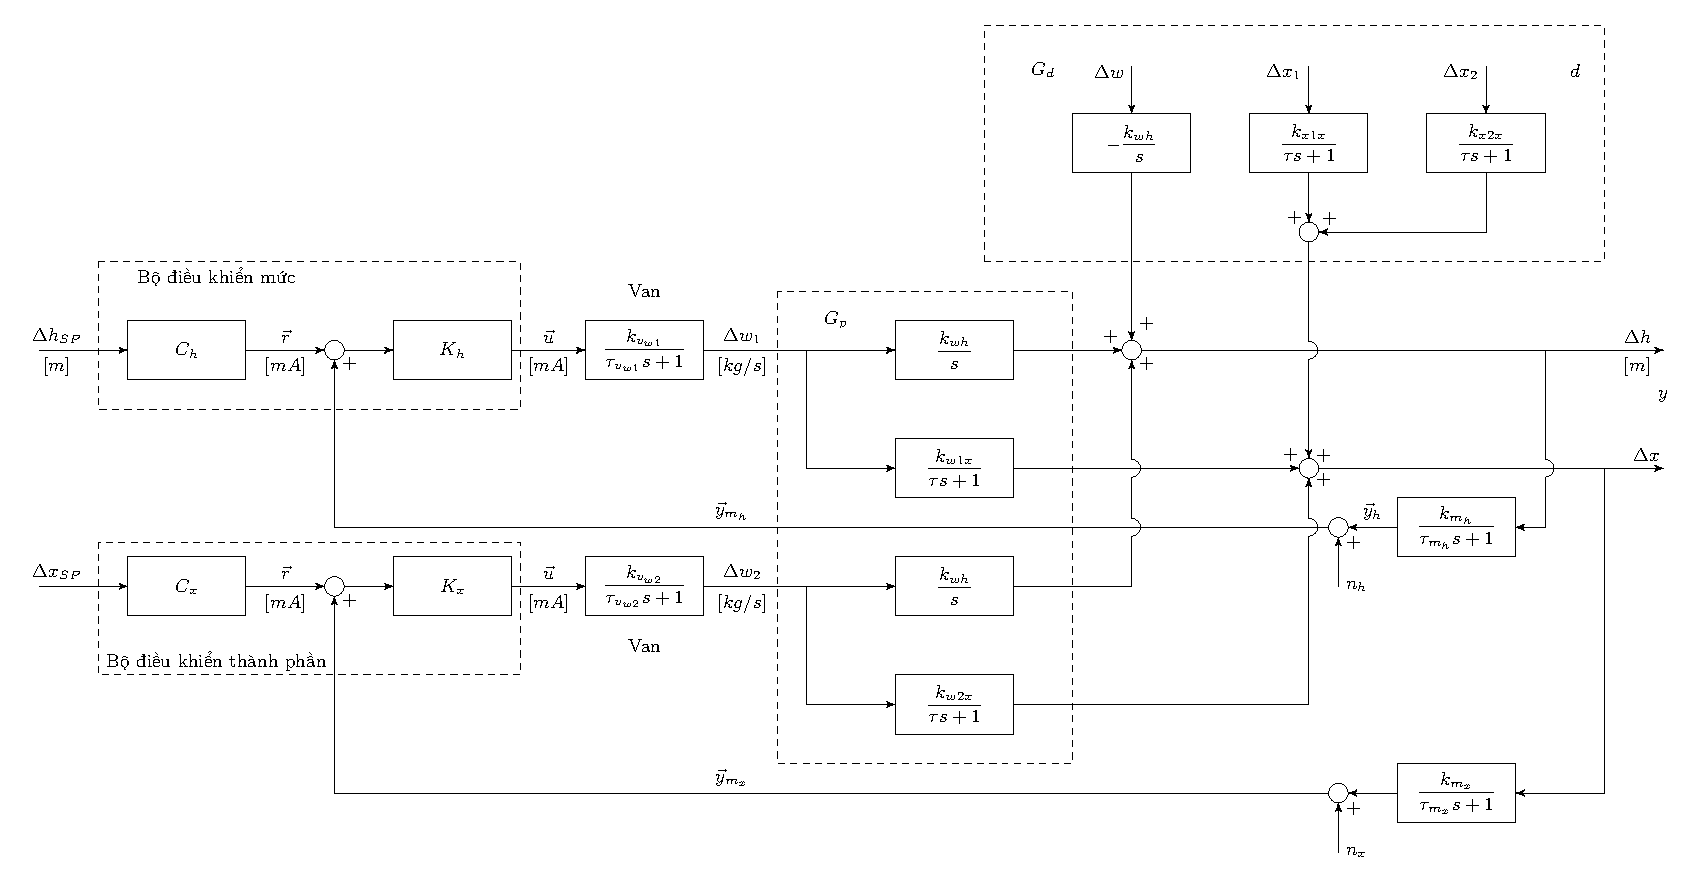
\includegraphics[scale=0.93]{section/mohinhhoalythuyet/images/binhchuachatlong-khuaytron-mohinh1-sodokhoi-cautrucdieukhienphanhoi}
            \end{center}
            \caption{Sơ đồ khối cho cấu trúc điều khiển phản hồi thiết bị khuấy trộn liên tục} \label{Fig:binhchuachatlong-khuaytron-sodokhoi-dieukhienphanhoi}
        \end{figure}
    \end{landscape}
